% Search for all the places that say "PUT SOMETHING HERE".

\documentclass[11pt]{article}
\usepackage{amsmath,textcomp,amssymb,graphicx,enumerate,hyperref,enumitem,mathtools,tikz-qtree,listings,chemformula,bm,graphicx,grffile,gensymb,physics,amssymb,datetime,siunitx}
\graphicspath{{/Users/jonathansun5/Documents/Fall 2017/MCB 166/Homeworks/Midterm/Screen Shot 2017-10-08 at 1.05.55 AM.png} {/Users/jonathansun5/Documents/Fall 2017/MCB 166/Homeworks/Midterm/Screen Shot 2017-10-08 at 2.21.48 AM.png} {/Users/jonathansun5/Documents/Fall 2017/MCB 166/Homeworks/Midterm/Screen Shot 2017-10-08 at 6.01.46 AM.png} {/Users/jonathansun5/Documents/Fall 2017/MCB 166/Homeworks/Midterm/Screen Shot 2017-10-10 at 5.14.12 AM.png} {/Users/jonathansun5/Documents/Fall 2017/MCB 166/Homeworks/Midterm/Screen Shot 2017-10-10 at 6.19.25 AM.png} {/Users/jonathansun5/Documents/Fall 2017/MCB 166/Homeworks/Midterm/Screen Shot 2017-10-10 at 8.07.09 AM.png} {/Users/jonathansun5/Documents/Fall 2017/MCB 166/Homeworks/Midterm/Screen Shot 2017-10-10 at 9.12.56 AM.png} {/Users/jonathansun5/Documents/Fall 2017/MCB 166/Homeworks/Midterm/Screen Shot 2017-10-10 at 10.23.32 AM.png} {/Users/jonathansun5/Documents/Fall 2017/MCB 166/Homeworks/Midterm/Screen Shot 2017-10-10 at 10.41.02 AM.png} {/Users/jonathansun5/Documents/Fall 2017/MCB 166/Homeworks/Midterm/Screen Shot 2017-10-10 at 10.51.13 AM.png}}

\makeatletter
\newcommand{\leqnos}{\tagsleft@true\let\veqno\@@leqno}
\newcommand{\reqnos}{\tagsleft@false\let\veqno\@@eqno}
\reqnos
\makeatother

\def\Name{Jonathan Sun}  % Your name
\def\SID{25020651}  % Your student ID number
\def\Homework{Midterm} % Number of Homework
\def\Session{Fall 2017}


\title{MCB166 --- \Session --- \Homework}
\author{\Name, SID \SID}
\markboth{MCB166 --- \Session --- \Homework --- \Name}{MCB166 --- \Session --- \Homework --- \Name}
\pagestyle{myheadings}
\newdate{date}{10}{10}{2017}
\date{\displaydate{date}}

\def\endproofmark{$\Box$}
\newenvironment{proof}{\par{\bf Proof:}}{\endproofmark\smallskip}

\usepackage[margin=1in]{geometry}



\begin{document}
\maketitle

\newpage
\begin{enumerate}[label=\arabic*.]
\item
Consider the simple cylindrical model of a \ch{K+} permeable ion channel shown in the figure.
\begin{enumerate}[label=\Alph*.]
\item
Starting with Fick’s first law and using the numbers given below, calculate the following for the \ch{K+} channel shown in the figure:
\begin{center}
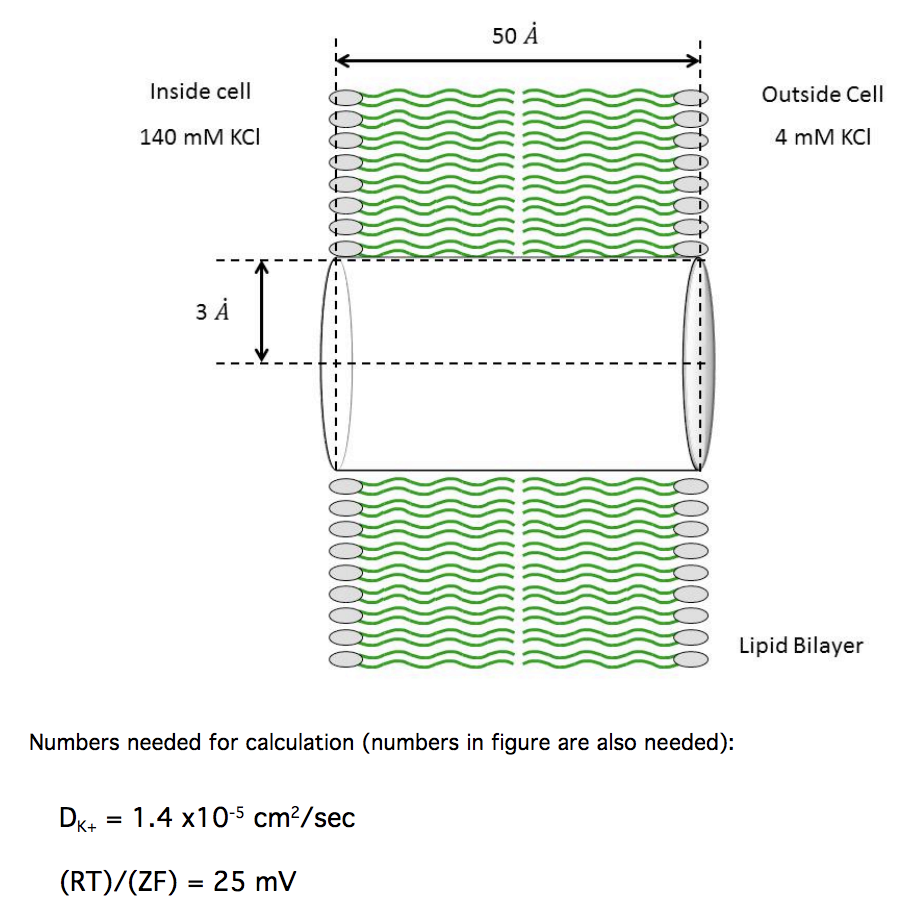
\includegraphics[width=0.75\textwidth]{/Users/jonathansun5/Documents/Fall 2017/MCB 166/Homeworks/Midterm/Screen Shot 2017-10-08 at 1.05.55 AM.png}
\end{center}
\begin{enumerate}[label=\arabic*.]
\item
The flux through the channel in ions/second.
\vspace*{1\baselineskip}
\\
To solve this problem, we start with:
\begin{align*}
J = -D \frac{\partial [C]} {\partial x}
\end{align*}
Using the values given, we get:
\begin{align*}
J = -\left(1.4 \times 10^{-5} \frac{\text{cm} ^ 2} {\text{s}}\right) \left(\frac{4 \text{mM} - 140 \text{mM}} {\SI{50}{\angstrom}}\right)
\end{align*}
\begin{align*}
J = -\left(1.4 \times 10^{-5} \frac{\text{cm} ^ 2} {\text{s}}\right) \left(\frac{- 136 \text{mM}} {\SI{50}{\angstrom}}\right)
\end{align*}
\begin{align*}
J = -\left(1.4 \times 10^{-5} \frac{\text{cm} ^ 2} {\text{s}}\right) \left(\frac{- 0.000136 \frac{\text{mol}} {\text{cm} ^ 3}} {50 \times 10 ^ {-8} \text{cm}}\right)
\end{align*}
\begin{align*}
J = 0.003808 \frac{\text{mol}} {\text{cm} ^ {2} \times \text{s}}
\end{align*}
I will multiply this by Avogadro's number $\left(6.023 \times 10 ^{23} \frac{\text{ions}} {\text{mol}}\right)$:
\begin{align*}
J = 0.003808 \frac{\text{mol}} {\text{cm} ^ {2} \times \text{s}} \times 6.023 \times 10 ^{23} \frac{\text{ions}} {\text{mol}}
\end{align*}
\begin{align*}
J \approx 2.2935584 \times 10 ^ {21} \frac{\text{ions}} {\text{cm} ^ {2} \times \text{s}}
\end{align*}
To calculate the flux through the channel in $\frac{\text{ions}} {\text{s}}$:
\begin{align*}
2.2935584 \times 10 ^ {21} \frac{\text{ions}} {\text{cm} ^ {2} \times \text{s}} \times \pi r ^ 2
\end{align*}
Since $r = \SI{3}{\angstrom}$:
\begin{align*}
= 2.2935584 \times 10 ^ {21} \frac{\text{ions}} {\text{cm} ^ {2} \times \text{s}} \times \pi \left(\SI{3}{\angstrom}\right) ^ 2
\end{align*}
\begin{align*}
= 2.2935584 \times 10 ^ {21} \frac{\text{ions}} {\text{cm} ^ {2} \times \text{s}} \times \pi \times 9 \times \left(\SI{1}{\angstrom}\right) ^ 2 \times \frac{\left(10 ^ {-8} \text{cm}\right) ^ 2} {\SI{1}{\angstrom} ^ 2}
\end{align*}
\begin{align*}
= 2.2935584 \times 10 ^ {21} \frac{\text{ions}} {\text{cm} ^ {2} \times \text{s}} \times \pi \times 9 \times 10 ^ {-16} \text{cm} ^ {2}
\end{align*}
\begin{align*}
\approx 6.4849 \times 10 ^ 6 \frac{\text{ions}} {\text{s}}
\end{align*}
Therefore, the flux through the channel would be approximately $6.4849 \times 10 ^ 6 \frac{\text{ions}} {\text{s}}$.



\newpage
\item
The single channel current.
\vspace*{1\baselineskip}
\\
To solve this problem, we start with $J = \frac{I} {A}$, where $J$ is the flux, $I$ is the current, and $A$ is the area of the circular part of the channel:
\begin{align*}
J = \frac{I} {A}
\end{align*}
\begin{align*}
I = J \times A
\end{align*}
Using the flux that we got from the question above and that $A = \pi r ^ 2$ where $r = \SI{3}{\angstrom}$, we get:
\begin{align*}
I =  0.003808 \frac{\text{mol}} {\text{cm} ^ {2} \times \text{s}} \times \pi r ^ 2
\end{align*}
\begin{align*}
I =  0.003808 \frac{\text{mol}} {\text{cm} ^ {2} \times \text{s}} \times \pi \times \left(\SI{3}{\angstrom}\right) ^ 2
\end{align*}
\begin{align*}
I =  0.003808 \frac{\text{mol}} {\text{cm} ^ {2} \times \text{s}} \times \pi \times 9 \times \left(\SI{1}{\angstrom}\right) ^ 2 \times \frac{\left(10 ^ {-8} \text{cm}\right) ^ 2} {\SI{1}{\angstrom} ^ 2}
\end{align*}
\begin{align*}
I =  0.003808 \frac{\text{mol}} {\text{cm} ^ {2} \times \text{s}} \times \pi \times 9 \times 10 ^ {-16} \text{cm} ^ {2}
\end{align*}
\begin{align*}
I \approx 1.07668663 \times 10 ^ {-17} \frac{\text{mol}} {\text{s}}
\end{align*}
To convert this into Amps, we have to multiply this by Faraday's Constant $\left(9.648 \times 10 ^ 4 \frac{\text{C}} {\text{mol}}\right)$:
\begin{align*}
I \approx 1.07668663 \times 10 ^ {-17} \frac{\text{mol}} {\text{s}} \times 9.648 \times 10 ^ 4 \frac{\text{C}} {\text{mol}}
\end{align*}
\begin{align*}
I \approx 1.03878726 \times 10 ^ {-12} \frac{\text{C}} {\text{s}} = 1.03878726 \times 10 ^ {-12} \text{A}
\end{align*}
Therefore, the current flowing through the \ch{K+} channel would be approximately $1.03878726 \times 10 ^ {-12} A$.



\newpage
\item
The single channel conductance, assuming that the channel is selective for potassium.
\vspace*{1\baselineskip}
\\
To solve this problem, we start with $G = \frac{I} {V}$, where $G$ is the conductance, $I$ is the current, and $V$ is the voltage:
\begin{align*}
G = \frac{I} {V}
\end{align*}
We also know that the membrane potential for this \ch{K+} ion channel is represented as:
\begin{align*}
E_{\ch{K}} = \frac{R T} {z F} \ln{\left(\frac{\ch{K_o}} {\ch{K_i}}\right)}
\end{align*}
\begin{align*}
E_{\ch{K}} = 25 \text{mV} \times \ln{\left(\frac{4 \text{mM}} {140 \text{mM}}\right)}
\end{align*}
\begin{align*}
E_{\ch{K}} = 25 \text{mV} \times \frac{1 \text{V}} {1000 \text{mV}} \times \ln{\left(\frac{4} {140}\right)}
\end{align*}
\begin{align*}
E_{\ch{K}} \approx -0.0888837015 \text{V}
\end{align*}
Plugging this and our current from the previous part into our equation for conductance we get:
\begin{align*}
G = \frac{I} {V}
\end{align*}
\begin{align*}
G = \frac{1.03878726 \times 10 ^ {-12} \text{A}} {-0.0888837015 \text{V}}
\end{align*}
\begin{align*}
G \approx -1.1687039 \times 10 ^ {-11} \frac{\text{A}} {\text{V}} = -1.1687039 \times 10 ^ {-11} \text{S}
\end{align*}
Therefore, the single channel conductance is $-1.1687039 \times 10 ^ {-11} \text{S}$.
\end{enumerate}



\newpage
\item
What other factors might need to be included in the above calculation to more accurately describe flux through an ion channel?
\vspace*{1\baselineskip}
\\
The drift flux from Ohm's law for drift can be included to more accurately describe flux through an ion channel. This is because flux is actually equivalent to the diffusion flux plus the drift flux, or $J = J_{Diffusion} + J_{Drift} = - \left(D \frac{\partial c} {\partial x} + zc\mu \frac{\partial V} {\partial x}\right)$.
\end{enumerate}



\newpage
\item
The figure below shows the equivalent circuit representation of a giant axon (as used in the Hodgkin-Huxley picture).
\begin{center}
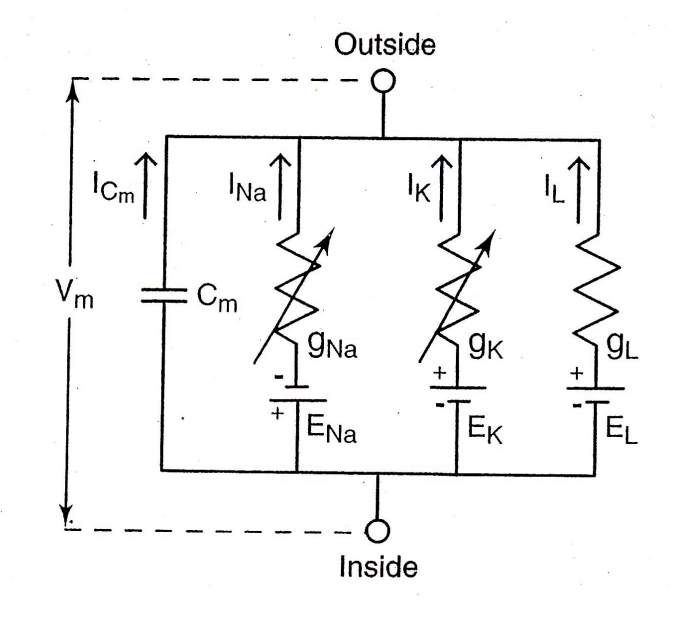
\includegraphics[width=0.75\textwidth]{/Users/jonathansun5/Documents/Fall 2017/MCB 166/Homeworks/Midterm/Screen Shot 2017-10-08 at 2.21.48 AM.png}
\end{center}
First we will consider the axon at rest, so that the three conductances are
in the ratio:
\begin{align*}
G_{\ch{K}} : G_{\ch{Cl}} : G_{\ch{Na}} = 1 : 0.1 : 0.03 \\
\text{assume } g_{\ch{L}} = g_{\ch{Cl}}\text{; } E_{\ch{L}} = E_{\ch{Cl}}
\end{align*}
We have not included the \ch{Na}-\ch{K} ATPase pump in the figure, but we will include it in a later problem. The arrows represent the voltage dependence of the conductances, which will also be used in a later question.
\begin{enumerate}[label=\alph*.]
\item
Derive a formula for the membrane resting potential in terms of the conductances, $G_{\ch{K}}$, $G_{\ch{Na}}$, $G_{\ch{Cl}}$ and the reversal potentials, $E_{\ch{K}}$, $E_{\ch{Na}}$, $E_{\ch{Cl}}$. That is, state the condition of membrane current for which the steady-state resting potential prevails.
\vspace*{1\baselineskip}
\\
To solve this problem, we start with:
\begin{align*}
I_{total} = C_m \frac{dV_m} {dt} + G_{\ch{K}} \left(V_m - E_{\ch{K}}\right) + G_{\ch{Na}} \left(V_m - E_{\ch{Na}}\right) + G_{\ch{Cl}} \left(V_m - E_{\ch{Cl}}\right) = 0
\end{align*}
\begin{align*}
G_{\ch{K}} \left(V_m - E_{\ch{K}}\right) + G_{\ch{Na}} \left(V_m - E_{\ch{Na}}\right) + G_{\ch{Cl}} \left(V_m - E_{\ch{Cl}}\right) = 0
\end{align*}
\begin{align*}
G_{\ch{K}} V_m - G_{\ch{K}} E_{\ch{K}} + G_{\ch{Na}} V_m - G_{\ch{Na}} E_{\ch{Na}} + G_{\ch{Cl}} V_m - G_{\ch{Cl}} E_{\ch{Cl}} = 0
\end{align*}
\begin{align*}
G_{\ch{K}} V_m + G_{\ch{Na}} V_m + G_{\ch{Cl}} V_m = G_{\ch{K}} E_{\ch{K}} + G_{\ch{Na}} E_{\ch{Na}} + G_{\ch{Cl}} E_{\ch{Cl}}
\end{align*}
\begin{align*}
V_m = \frac{G_{\ch{K}} E_{\ch{K}} + G_{\ch{Na}} E_{\ch{Na}} + G_{\ch{Cl}} E_{\ch{Cl}}} {G_{\ch{K}} + G_{\ch{Na}} + G_{\ch{Cl}}}
\end{align*}



\newpage
\item
Under steady-state conditions, the formula you have derived (or looked up in the notes) gives the membrane potential in terms of concentrations and conductances. We will now consider an axon of a marine invertebrate, such as the squid. At rest, the only permeable ions are \ch{Na+}, \ch{K+}, and \ch{Cl-}. The major internal and external ion concentrations are:
\begin{align*}
[\ch{K}]_o = 20 \text{mM}\text{; }[\ch{Na}]_o = 490 \text{mM}\text{; }[\ch{Cl}]_o = 500 \text{mM} \\
[\ch{K}]_i = 400 \text{mM}\text{; }[\ch{Na}]_i = 50 \text{mM}\text{; }[\ch{Cl}]_i = 32.8 \text{mM}
\end{align*}
Assuming the three pathways are perfectly selective, calculate the reversal potentials, $E_{\ch{K}}$, $E_{\ch{Na}}$, $E_{\ch{Cl}}$. You may use the value $k T/e = 25.9 \text{mV}$ at $T =300 \text{K}$ $\left(23 ^{\circ}\text{C}\right)$, normal room temperature.
\vspace*{1\baselineskip}
\\
To solve this problem, I will use the Nernst Equation to find $E_{\ch{K}}$, $E_{\ch{Na}}$, $E_{\ch{Cl}}$:
\vspace*{1\baselineskip}
\\
For $E_{\ch{K}}$:
\begin{align*}
E_{\ch{K}} = \frac{R T} {z F} \ln{\left(\frac{[\ch{K}]_o} {[\ch{K}]_i}\right)}
\end{align*}
Since $\frac{R T} {F} = \frac{k T} {e}$ and $\frac{k T} {e} = 25.9 \text{mV}$:
\begin{align*}
E_{\ch{K}} = \frac{k T} {ze} \ln{\left(\frac{[\ch{K}]_o} {[\ch{K}]_i}\right)}
\end{align*}
Since $z$ is the valency of the \ch{K+} ion, which is $1$:
\begin{align*}
E_{\ch{K}} = 25.9 \text{mV} \times \ln{\left(\frac{20 \text{mM}} {400 \text{mM}}\right)}
\end{align*}
\begin{align*}
E_{\ch{K}} \approx -77.59 \text{mV}
\end{align*}
\vspace*{1\baselineskip}
\\
For $E_{\ch{Na}}$:
\begin{align*}
E_{\ch{Na}} = \frac{R T} {z F} \ln{\left(\frac{[\ch{Na}]_o} {[\ch{Na}]_i}\right)}
\end{align*}
Since $\frac{R T} {F} = \frac{k T} {e}$ and $\frac{k T} {e} = 25.9 \text{mV}$:
\begin{align*}
E_{\ch{Na}} = \frac{k T} {ze} \ln{\left(\frac{[\ch{Na}]_o} {[\ch{Na}]_i}\right)}
\end{align*}
Since $z$ is the valency of the \ch{Na+} ion, which is $1$:
\begin{align*}
E_{\ch{Na}} = 25.9 \text{mV} \times \ln{\left(\frac{490 \text{mM}} {50 \text{mM}}\right)}
\end{align*}
\begin{align*}
E_{\ch{Na}} \approx 59.11 \text{mV}
\end{align*}
\vspace*{1\baselineskip}
\\
For $E_{\ch{Cl}}$:
\begin{align*}
E_{\ch{Cl}} = \frac{R T} {z F} \ln{\left(\frac{[\ch{Cl}]_o} {[\ch{Cl}]_i}\right)}
\end{align*}
Since $\frac{R T} {F} = \frac{k T} {e}$ and $\frac{k T} {e} = 25.9 \text{mV}$:
\begin{align*}
E_{\ch{Cl}} = \frac{k T} {ze} \ln{\left(\frac{[\ch{Cl}]_o} {[\ch{Cl}]_i}\right)}
\end{align*}
Since $z$ is the valency of the \ch{Cl-} ion, which is $-1$:
\begin{align*}
E_{\ch{Cl}} = -25.9 \text{mV} \times \ln{\left(\frac{500 \text{mM}} {32.8 \text{mM}}\right)}
\end{align*}
\begin{align*}
E_{\ch{Cl}} \approx -70.56 \text{mV}
\end{align*}
Therefore, the reversal potentials for \ch{K}, \ch{Na}, \ch{Cl} are $-77.59 \text{mV}$, $59.11 \text{mV}$, and $-70.56 \text{mV}$ respectively.



\newpage
\item
Calculate the membrane potential at room temperature.
\vspace*{1\baselineskip}
\\
To solve this problem, I will use the equation I got from part (a), the ratios of the conductances, and the values from part (b):
\begin{align*}
V_m = \frac{G_{\ch{K}} E_{\ch{K}} + G_{\ch{Na}} E_{\ch{Na}} + G_{\ch{Cl}} E_{\ch{Cl}}} {G_{\ch{K}} + G_{\ch{Na}} + G_{\ch{Cl}}}
\end{align*}
\begin{align*}
V_m \approx \frac{1 \times -77.59 \text{mV} + 0.03 \times 59.11 \text{mV} + 0.1 \times -70.56 \text{mV}} {1 + 0.03 + 0.1}
\end{align*}
\begin{align*}
V_m \approx \frac{-82.87 \text{mV}} {1.13}
\end{align*}
\begin{align*}
V_m \approx -73.34 \text{mV}
\end{align*}
Therefore, the membrane potential at room temperature is $-73.34 \text{mV}$.



\newpage
\item
In reality, this creature lives at the chilly ocean temperature of $6.3 ^{\circ}\text{C}$. Recalculate the membrane potential for this more natural condition. 
\vspace*{1\baselineskip}
\\
To solve this problem, I need to find the new $\frac{R T} {F}$ with $T = 6.3 ^{\circ}\text{C} = 279.45 \text{K}$:
\begin{align*}
\frac{R T} {F} = \frac{8.314 \frac{\text{J}} {\text{K} \times \text{mol}} \times 279.45 \text{K}} {9.648 \times 10 ^ 4 \frac{\text{C}} {\text{mol}}} \approx 0.0240811287 \frac{\text{J}} {\text{C}} \approx 0.0240811287 \text{V} \approx 24.08 \text{mV}
\end{align*}
Next, I need the recalculate the Nernst Equation to find $E_{\ch{K}}$, $E_{\ch{Na}}$, $E_{\ch{Cl}}$:
\vspace*{1\baselineskip}
\\
For $E_{\ch{K}}$:
\begin{align*}
E_{\ch{K}} = \frac{R T} {z F} \ln{\left(\frac{[\ch{K}]_o} {[\ch{K}]_i}\right)}
\end{align*}
Since $z$ is the valency of the \ch{K+} ion, which is $1$:
\begin{align*}
E_{\ch{K}} = 24.08 \text{mV} \times \ln{\left(\frac{20 \text{mM}} {400 \text{mM}}\right)}
\end{align*}
\begin{align*}
E_{\ch{K}} \approx -72.14 \text{mV}
\end{align*}
\vspace*{1\baselineskip}
\\
For $E_{\ch{Na}}$:
\begin{align*}
E_{\ch{Na}} = \frac{R T} {z F} \ln{\left(\frac{[\ch{Na}]_o} {[\ch{Na}]_i}\right)}
\end{align*}
Since $z$ is the valency of the \ch{Na+} ion, which is $1$:
\begin{align*}
E_{\ch{Na}} = 24.08 \text{mV} \times \ln{\left(\frac{490 \text{mM}} {50 \text{mM}}\right)}
\end{align*}
\begin{align*}
E_{\ch{Na}} \approx 54.96 \text{mV}
\end{align*}
\vspace*{1\baselineskip}
\\
For $E_{\ch{Cl}}$:
\begin{align*}
E_{\ch{Cl}} = \frac{R T} {z F} \ln{\left(\frac{[\ch{Cl}]_o} {[\ch{Cl}]_i}\right)}
\end{align*}
Since $z$ is the valency of the \ch{Cl-} ion, which is $-1$:
\begin{align*}
E_{\ch{Cl}} = -24.08 \text{mV} \times \ln{\left(\frac{500 \text{mM}} {32.8 \text{mM}}\right)}
\end{align*}
\begin{align*}
E_{\ch{Cl}} \approx -65.60 \text{mV}
\end{align*}
Recalculating the membrane potential gives me:
\begin{align*}
V_m = \frac{G_{\ch{K}} E_{\ch{K}} + G_{\ch{Na}} E_{\ch{Na}} + G_{\ch{Cl}} E_{\ch{Cl}}} {G_{\ch{K}} + G_{\ch{Na}} + G_{\ch{Cl}}}
\end{align*}
\begin{align*}
V_m \approx \frac{1 \times -72.14 \text{mV} + 0.03 \times 54.96 \text{mV} + 0.1 \times -65.60 \text{mV}} {1 + 0.03 + 0.1}
\end{align*}
\begin{align*}
V_m \approx \frac{-77.05 \text{mV}} {1.13}
\end{align*}
\begin{align*}
V_m \approx -68.19 \text{mV}
\end{align*}
Therefore, the membrane potential at $6.3 ^{\circ}\text{C}$ is $-68.19 \text{mV}$.



\newpage
\item
At the peak of the action potential, there is a $45$-fold increase in the sodium conductance with no change in potassium or chloride conductance. What potential is reached at peak activity? How does this compare with the sodium Nernst potential for the given concentrations? What is the amplitude of the action potential (from rest)?
\vspace*{1\baselineskip}
\\
To solve this problem, I will change the ratio of the conductance for sodium from $0.03$ to $1.35$ (since $0.03 \times 45 = 1.35$) to solve for the potential at the peak activity at room temperature:
\begin{align*}
V_m = \frac{G_{\ch{K}} E_{\ch{K}} + G_{\ch{Na}} E_{\ch{Na}} + G_{\ch{Cl}} E_{\ch{Cl}}} {G_{\ch{K}} + G_{\ch{Na}} + G_{\ch{Cl}}}
\end{align*}
\begin{align*}
V_m \approx \frac{1 \times -77.59 \text{mV} + 1.35 \times 59.11 \text{mV} + 0.1 \times -70.56 \text{mV}} {1 + 1.35 + 0.1}
\end{align*}
\begin{align*}
V_m \approx \frac{-4.8475 \text{mV}} {2.45}
\end{align*}
\begin{align*}
V_m \approx -1.98 \text{mV}
\end{align*}
Therefore, the potential at peak activity at room temperature is $-1.98 \text{mV}$. This makes the potential closer to the sodium Nernst potential, which is $59.11 \text{mV}$. The amplitude of the action potential from rest is $71.36 \text{mV}$ since this is the difference between $-1.98 \text{mV}$ and $-73.34 \text{mV}$.
\end{enumerate}



\newpage
\item
Now we wish to correct the membrane potential for the presence of a \ch{Na}-\ch{K} ATPase pump. This equivalent circuit has two parallel constant-current sources, $I_{P-\ch{Na}}$ and $I_{P-\ch{K}}$. This is an electrogenic pump defined by:
\begin{align*}
\text{(1) } I_{P-\ch{Na}} = - \frac{3} {2} I_{P-\ch{K}}
\end{align*}
The three leak currents are given by:
\begin{align*}
\text{(2) } I_{L-\ch{K}} = G_{\ch{K}} \left(V - E_{\ch{K}}\right) \text{, (3) } I_{L-\ch{Na}} = G_{\ch{Na}} \left(V - E_{\ch{Na}}\right) \text{, (4) } I_{L-\ch{Cl}} = G_{\ch{Cl}} \left(V - E_{\ch{Cl}}\right).
\end{align*}
\begin{enumerate}[label=(\alph*)]
\item
State the conditions for the membrane to be in ionic equilibrium in the presence of the pump. In question $2$, the total current was set equal to zero. Now the individual ionic species must be in equilibrium too. How do these conditions change the three reversal potentials? Are they still equal to the Nernst potentials for the individual ions? (hint: the answer is not the same for all of the ions).
\vspace*{1\baselineskip}
\\
For the membrane to be in ionic equilibrium in the presence of the pump, the net currents for each of the ion types need to equal to $0$.
\vspace*{1\baselineskip}
\\
The three conditions must be met:
\begin{align*}
\left\{
\begin{array}{l}
	I_{\ch{K}-pump} + I_{\ch{K}-leak} = 0 \\
	I_{\ch{Na}-pump} + I_{\ch{Na}-leak} = 0 \\
	I_{\ch{Cl}-leak} = 0
\end{array}
\right.
\end{align*}
From the conditions above, we get:
\begin{align*}
\left\{
\begin{array}{l}
	G_{\ch{K}} \left(V - E_{\ch{K}}\right) = - I_{\ch{K}-pump} \\
	G_{\ch{Na}} \left(V - E_{\ch{Na}}\right) = - I_{\ch{Na}-pump} \\
	G_{\ch{Cl}} \left(V - E_{\ch{Cl}}\right) = 0
\end{array}
\right.
\end{align*}
\begin{align*}
\Rightarrow \left\{
\begin{array}{l}
	G_{\ch{K}} V - G_{\ch{K}} E_{\ch{K}} = - I_{\ch{K}-pump} \\
	G_{\ch{Na}} V - G_{\ch{Na}} E_{\ch{Na}} = - I_{\ch{Na}-pump} \\
	G_{\ch{Cl}} V - G_{\ch{Cl}} E_{\ch{Cl}} = 0
\end{array}
\right. 
\end{align*}
\begin{align*}
\Rightarrow \left\{
\begin{array}{l}
	G_{\ch{K}} E_{\ch{K}} = G_{\ch{K}} V + I_{\ch{K}-pump} \\
	G_{\ch{Na}} E_{\ch{Na}} = G_{\ch{Na}} V + I_{\ch{Na}-pump} \\
	G_{\ch{Cl}} E_{\ch{Cl}} = G_{\ch{Cl}} V
\end{array}
\right.
\end{align*}
Thus, we get:
\begin{align*}
\Rightarrow \left\{
\begin{array}{l}
	E_{\ch{K}} = \frac{G_{\ch{K}} V + I_{\ch{K}-pump}} {G_{\ch{K}}} \\
	E_{\ch{Na}} = \frac{G_{\ch{Na}} V + I_{\ch{Na}-pump}} {G_{\ch{Na}}} \\
	E_{\ch{Cl}} = V
\end{array}
\right.
\end{align*}
\begin{align*}
\Rightarrow \left\{
\begin{array}{l}
	E_{\ch{K}} = \frac{G_{\ch{K}} V - \frac{2} {3} I_{\ch{K}-pump}} {G_{\ch{K}}} \\
	E_{\ch{Na}} = \frac{G_{\ch{Na}} V - \frac{3} {2} I_{\ch{K}-pump}} {G_{\ch{Na}}} \\
	E_{\ch{Cl}} = V
\end{array}
\right.
\end{align*}
The reversal potential for \ch{Na+} will become more positive since the pump will pump out \ch{Na+}, the reversal potential for \ch{K+} will become more negative since the pump will pump in \ch{K+}, and the reversal potential for \ch{Cl-} will remain the same. Therefore, the reversal potentials for \ch{Na+} and \ch{K+} will not equal the Nernst potentials for the individual ions.



\newpage
\item
Derive a formula for the membrane potential corrected for the pump. The derivation follows what was done in class notes for the constant-field model, but now we use the linear current-voltage relations of Eqns. $2$ –- $4$ (as in PSet \#$2$, Problem \#$3$). The result is surprisingly simple.
\vspace*{1\baselineskip}
\\
To solve this problem, we start with:
\begin{align*}
I_{total} = I_{\ch{Na}-leak} + I_{\ch{Na}-pump} + I_{\ch{K}-leak} + I_{\ch{K}-pump} + I_{\ch{Cl}-leak} = 0
\end{align*}
\begin{align*}
I_{\ch{Na}-leak} + \left(-\frac{3} {2} I_{\ch{K}-pump}\right) + I_{\ch{K}-leak} + I_{\ch{K}-pump} + I_{\ch{Cl}-leak} = 0
\end{align*}
\begin{align*}
I_{\ch{Na}-leak} - \frac{1} {2} I_{\ch{K}-pump} + I_{\ch{K}-leak} + I_{\ch{Cl}-leak} = 0
\end{align*}
\begin{align*}
I_{\ch{Na}-leak} + \frac{1} {2} I_{\ch{K}-leak} + I_{\ch{K}-leak} + I_{\ch{Cl}-leak} = 0
\end{align*}
\begin{align*}
I_{\ch{Na}-leak} + \frac{3} {2} I_{\ch{K}-leak} + I_{\ch{Cl}-leak} = 0
\end{align*}
This equation can be rewritten as:
\begin{align*}
G_{\ch{Na}} \left(V - E_{\ch{Na}}\right) + \frac{3} {2} G_{\ch{K}} \left(V - E_{\ch{K}}\right) + G_{\ch{Cl}} \left(V - E_{\ch{Cl}}\right) = 0
\end{align*}
\begin{align*}
G_{\ch{Na}} V - G_{\ch{Na}} E_{\ch{Na}} + \frac{3} {2} G_{\ch{K}} V - \frac{3} {2} G_{\ch{K}} E_{\ch{K}} + G_{\ch{Cl}} V - G_{\ch{Cl}} E_{\ch{Cl}} = 0
\end{align*}
\begin{align*}
G_{\ch{Na}} V + \frac{3} {2} G_{\ch{K}} V + G_{\ch{Cl}} V = G_{\ch{Na}} E_{\ch{Na}} + \frac{3} {2} G_{\ch{K}} E_{\ch{K}} + G_{\ch{Cl}} E_{\ch{Cl}}
\end{align*}
\begin{align*}
V = \frac{G_{\ch{Na}} E_{\ch{Na}} + \frac{3} {2} G_{\ch{K}} E_{\ch{K}} + G_{\ch{Cl}} E_{\ch{Cl}}} {G_{\ch{Na}} + \frac{3} {2} G_{\ch{K}} + G_{\ch{Cl}}}
\end{align*}



\newpage
\item
Calculate the resting potential at room temperature when the pump is operative. Does the pump depolarize or hyperpolarize the membrane potential? Explain your answer.
\vspace*{1\baselineskip}
\\
Since this takes place at room temperature, I will use the conductance rations, $E_{\ch{K}} \approx -77.59 \text{mV}$, $E_{\ch{Na}} \approx 59.11 \text{mV}$, and $E_{\ch{Cl}} \approx -70.56 \text{mV}$ from $2$(b) as well as the equation above:
\begin{align*}
V = \frac{G_{\ch{Na}} E_{\ch{Na}} + \frac{3} {2} G_{\ch{K}} E_{\ch{K}} + G_{\ch{Cl}} E_{\ch{Cl}}} {G_{\ch{Na}} + \frac{3} {2} G_{\ch{K}} + G_{\ch{Cl}}}
\end{align*}
\begin{align*}
V = \frac{0.03 \times 59.11 \text{mV} + \frac{3} {2} \times 1 \times -77.59 \text{mV} + 0.1 \times -70.56 \text{mV}} {0.03 + \frac{3} {2} \times 1 + 0.1}
\end{align*}
\begin{align*}
V = \frac{-121.67 \text{mV}} {1.63}
\end{align*}
\begin{align*}
V_m \approx -74.64 \text{mV}
\end{align*}
Therefore, the resting potential at room temperature when the pump is operative is $-74.64 \text{mV}$. Since this process generates a net outward current by pumping out more positive charge than it takes in and thus hyperpolarizes the membrane potential.



\newpage
\item
In the worked example in Pset $2$, we calculated the membrane potential (with pump on) but we ignored the \ch{Cl-} current. Recalculate $V_{\text{rest}}$ without the \ch{Cl-} terms (but with the pump on). The answer may surprise you. Explain why despite the relatively high permeability to \ch{Cl-} ions, ignoring the \ch{Cl-} terms has so little effect.
\vspace*{1\baselineskip}
\\
Since this takes place at room temperature, I will use the conductance rations, $E_{\ch{K}} \approx -77.59 \text{mV}$, $E_{\ch{Na}} \approx 59.11 \text{mV}$ from $2$(b) as well as the equation above except this time ignoring \ch{Cl-}:
\begin{align*}
V = \frac{G_{\ch{Na}} E_{\ch{Na}} + \frac{3} {2} G_{\ch{K}} E_{\ch{K}}} {G_{\ch{Na}} + \frac{3} {2} G_{\ch{K}}}
\end{align*}
\begin{align*}
V = \frac{0.03 \times 59.11 \text{mV} + \frac{3} {2} \times 1 \times -77.59 \text{mV}} {0.03 + \frac{3} {2} \times 1}
\end{align*}
\begin{align*}
V = \frac{-114.57 \text{mV}} {1.53}
\end{align*}
\begin{align*}
V_m \approx -74.91 \text{mV}
\end{align*}
The resting potential at room temperature when the pump is operative while disregarding \ch{Cl-} is $-74.91 \text{mV}$. The difference between the resting potential with and withough \ch{Cl-} is only $0.27 \text{mV}$, which is very insignificant. Therefore, despite the relatively high permeability to \ch{Cl-} ions, ignoring the \ch{Cl-} terms has so little effect.
\end{enumerate}



\newpage
\item
\underline{Voltage Clamp.}
\vspace*{1\baselineskip}
\\
Under voltage-clamp conditions, the membrane is depolarized from rest by a $60$ mV step of potential of $5$ msec duration ($60$ mV positive to the resting potential). The figure shows the ionic current that flows in response to this pulse.
\begin{center}
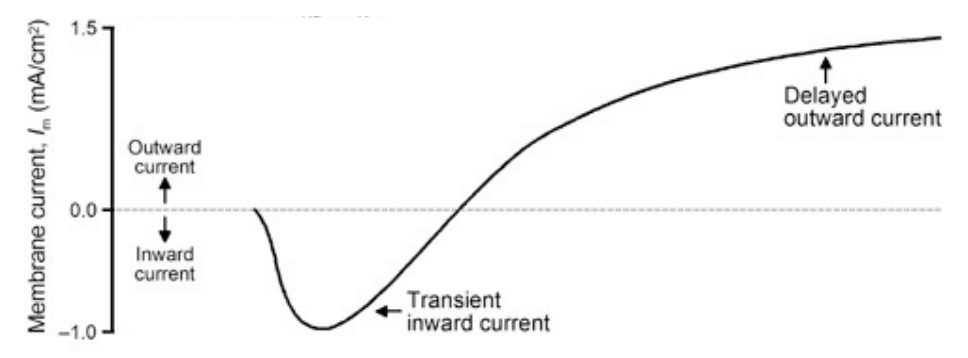
\includegraphics[width=0.75\textwidth]{/Users/jonathansun5/Documents/Fall 2017/MCB 166/Homeworks/Midterm/Screen Shot 2017-10-08 at 6.01.46 AM.png}
\end{center}
\begin{enumerate}[label=(\alph*)]
\item
Sketch the individual \ch{Na} and \ch{K} components of the current, and describe a way by which the current can be separated into these two components. (There is more than one way.)
\begin{center}
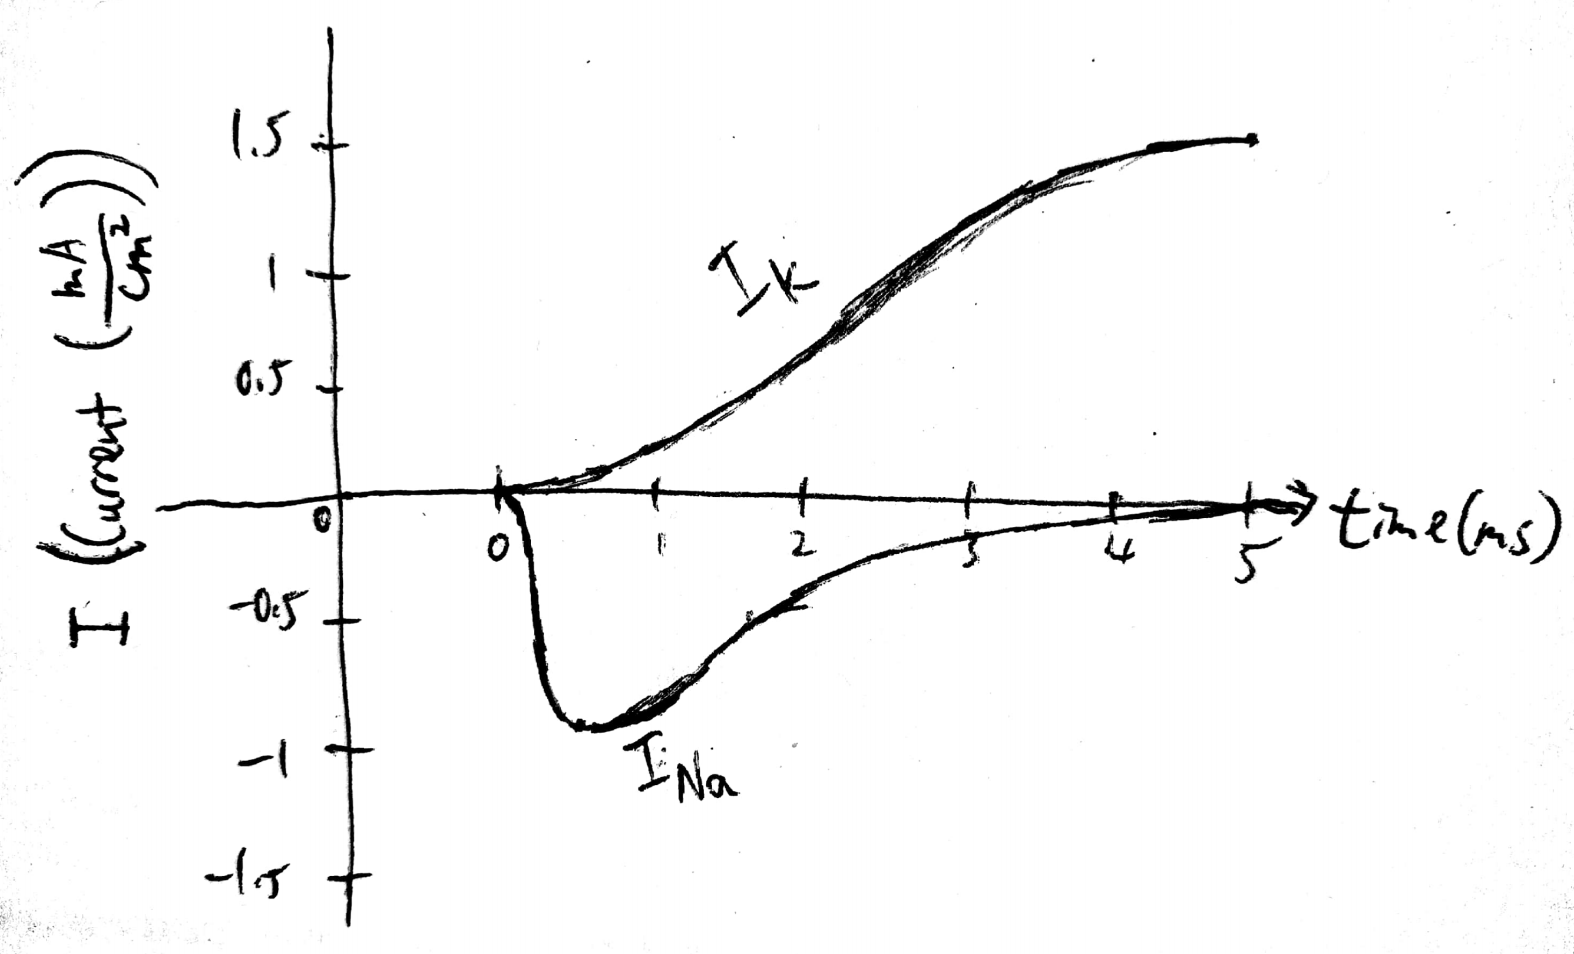
\includegraphics[width=0.75\textwidth]{/Users/jonathansun5/Documents/Fall 2017/MCB 166/Homeworks/Midterm/Screen Shot 2017-10-10 at 5.14.12 AM.png}
\end{center}
The current can be separated into individual \ch{Na+} and \ch{K+} components by the two ways. For the \ch{Na+}, one can remove the extracellular \ch{Na+} or add tetrodotoxin (TTX), which blocks \ch{Na+} channels, to eliminate the early transient inward current mediated by \ch{Na+} channels. For the \ch{K+}, one can remove the intracellular \ch{K+} or add tetraethylammonium (TEA), which blocks \ch{K+} channels, to eliminate the late outward current mediated by \ch{K+} channels.



\newpage
\item
Sketch the two components of time-dependent conductance, $g_{\ch{Na}}(t)$ and $g_{\ch{K}}(t)$, corresponding to the currents, and explain how the conductances are determined experimentally.
\begin{center}
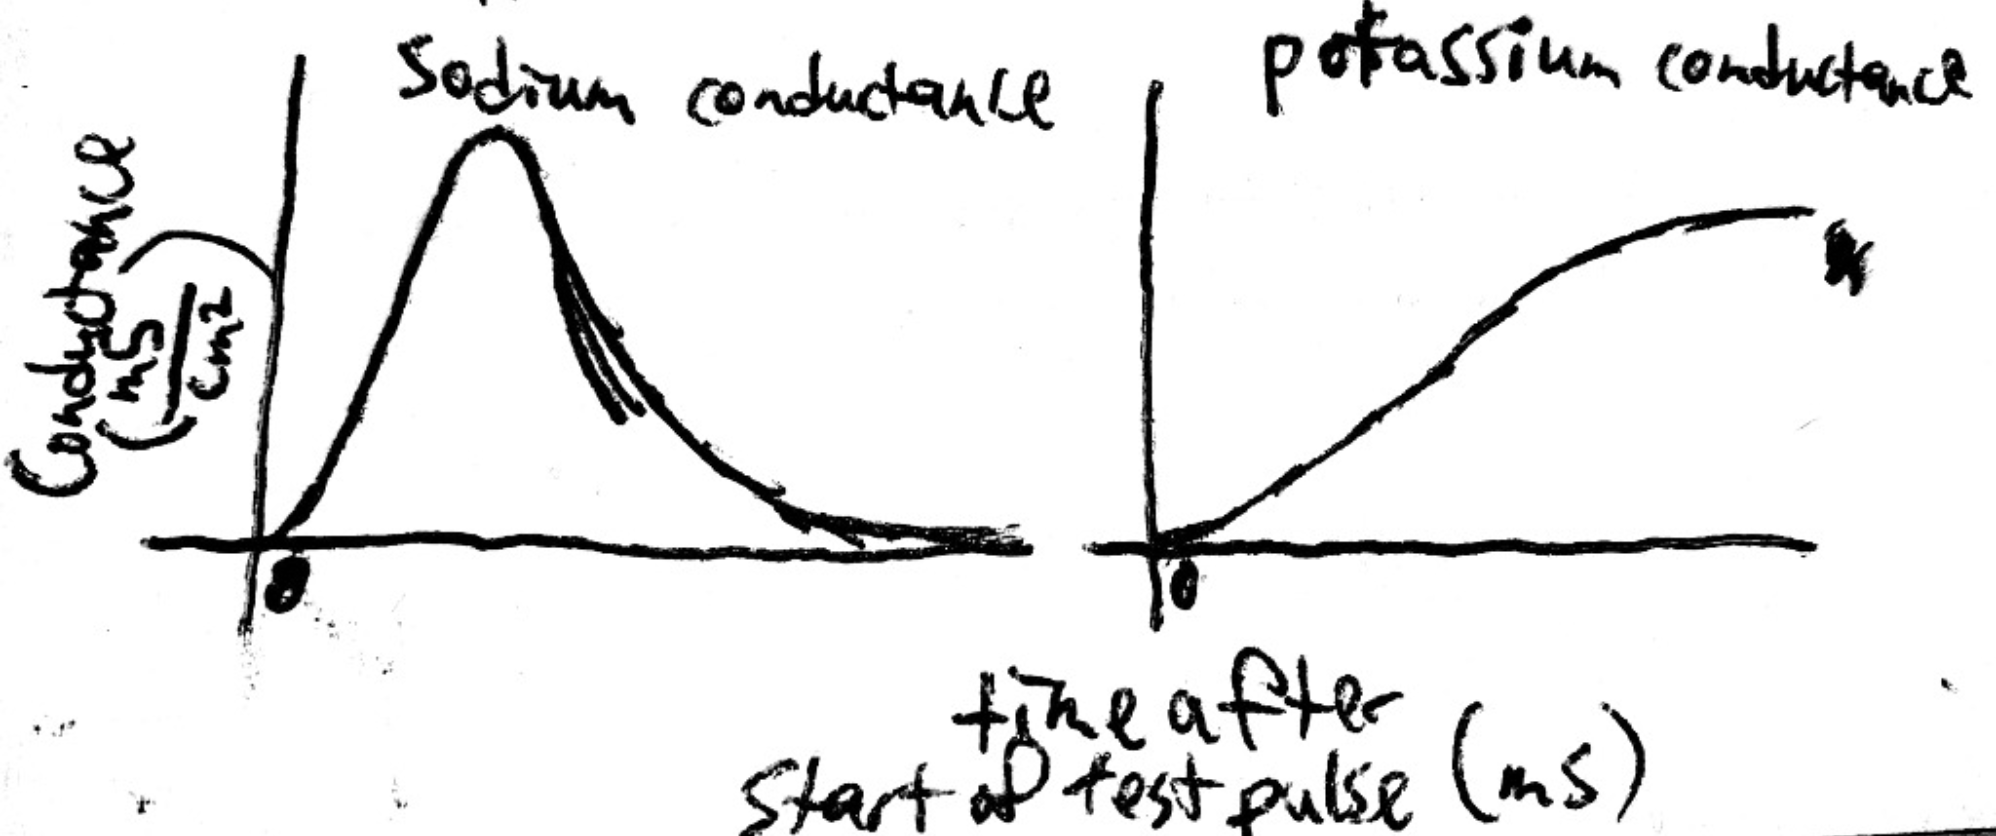
\includegraphics[width=0.75\textwidth]{/Users/jonathansun5/Documents/Fall 2017/MCB 166/Homeworks/Midterm/Screen Shot 2017-10-10 at 6.19.25 AM.png}
\end{center}
The conductances are determined experimentally using the same methods described above to get the graph of the currents for \ch{Na+} and \ch{K+}. Dividing the current for \ch{Na+} by $V - E_{\ch{Na}}$ and the current for \ch{K+} by $V - E_{\ch{K}}$ will give the values for $g_{\ch{Na}}(t)$ and $g_{\ch{K}}(t)$.



\newpage
\item
Explain in a short paragraph how the time-dependent conductances observed experimentally lead to the Hodgkin-Huxley gating variables $m$, $h$, and $n$. 
\vspace*{1\baselineskip}
\\
When Hodgkin and Huxley did the experiment, they proposed that the conductances were controlled by gating particles so they proposed that $g_{\ch{Na}}(V, t) = Y_{\ch{Na}}(V, t) \bar{g}_{\ch{Na}}$ and $g_{\ch{K}}(V, t) = Y_{\ch{K}}(V, t) \bar{g}_{\ch{K}}$ where $Y_{\ch{Na}}$ and $Y_{\ch{K}}$ are between $0$ and $1$. From this, they found that $Y_{\ch{Na}}$ and $Y_{\ch{K}}$ follow power functions of the exponential so they proposed $g_{\ch{Na}}(V, t) = Y_{\ch{Na}}(V, t) \bar{g}_{\ch{Na}} = m ^ 3 h \bar{g}_{\ch{Na}}$ and $g_{\ch{K}}(V, t) = Y_{\ch{K}}(V, t) \bar{g}_{\ch{K}} = n ^ 4 \bar{g}_{\ch{K}}$. In other words, they needed functions that fit the data and the function that fits the data have sigmoid curve (S--shape), which can be represented by the exponential.



\newpage
\item
Why are the gating variables $m$ and $n$ raised to powers in the Hodgkin-Huxley description? Explain why the on response to a depolarizing pulse exhibits a time delay and the off transient does not. You can explain things in terms of the concerted action of gating subunits in opening a channel.
\vspace*{1\baselineskip}
\\
As stated above, they found that the data follow power functions of the exponential, since the data plot showed the sigmoid curve (S--shape). So, the gating variable $m$ was raised to the power of $3$ and $n$ was raised to the power of $4$. The on response to a depolarizing pulse exhibits a time delay and the off transient does not because $n$ and $m$ are activated by depolarization but $h$ is inactivated by depolarization due to the boundary conditions for each of the variables based on the time ($h_0 > h_\infty$, $n_\infty > n_0$, $m_\infty > m_0$).
\end{enumerate}



\newpage
\item
\underline{Action Potentials and Propagation.}
\begin{enumerate}[label=(\alph*)]
\item
What happens during an action potential to make the membrane potential increase regeneratively? You may describe this process in terms of a cycle of events, but also explain the regenerative cycle in a few short sentences.
\begin{center}
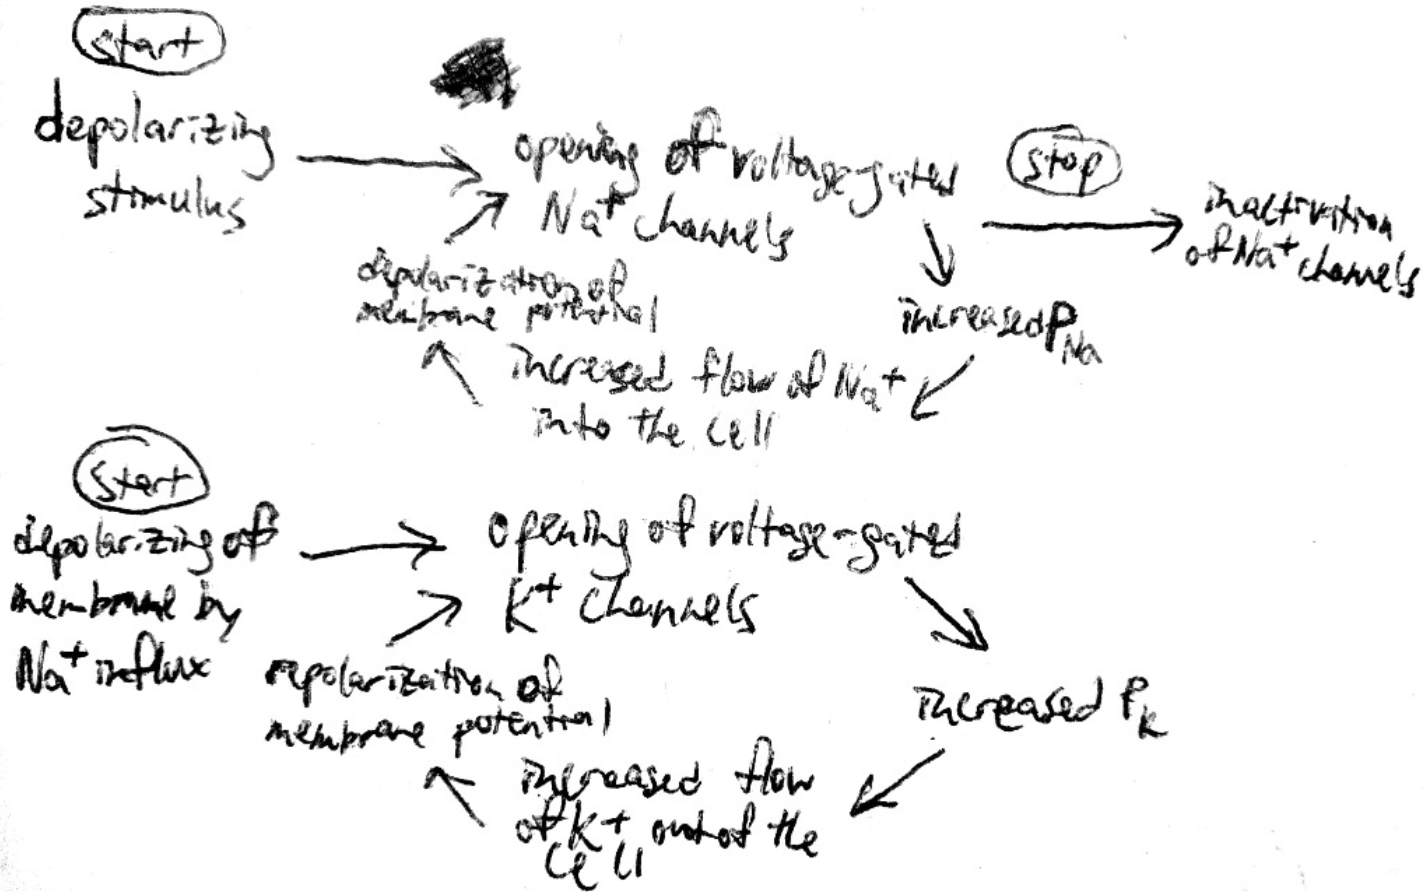
\includegraphics[width=0.75\textwidth]{/Users/jonathansun5/Documents/Fall 2017/MCB 166/Homeworks/Midterm/Screen Shot 2017-10-10 at 10.23.32 AM.png}
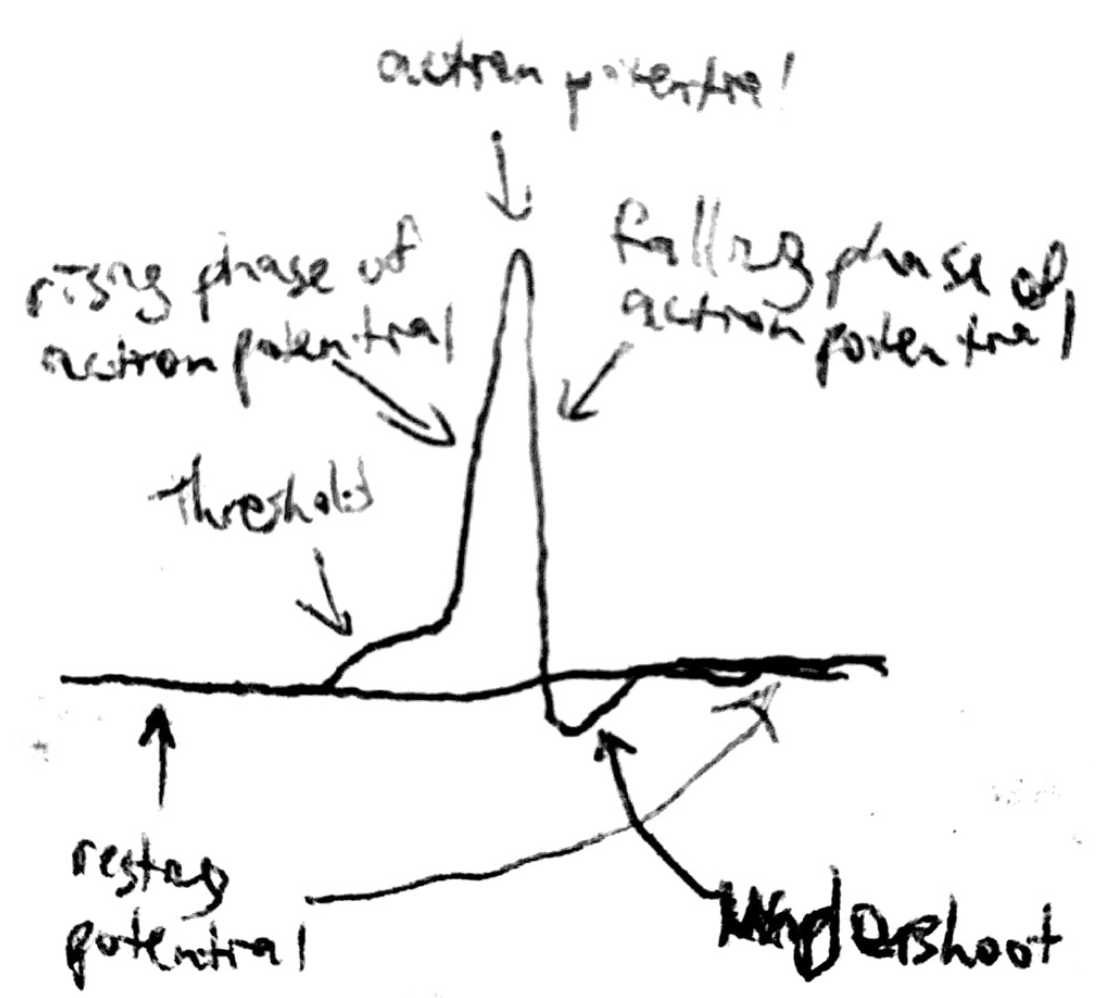
\includegraphics[width=0.5\textwidth]{/Users/jonathansun5/Documents/Fall 2017/MCB 166/Homeworks/Midterm/Screen Shot 2017-10-10 at 10.41.02 AM.png}
\end{center}

The membrane potential first starts at the resting potential until depolarization and the rising phase of the action potential happens, where sodium ions flood the cell because of the opening of sodium channels. During this time, the membrane potential increases. Once this reaches the action potential, the falling phase of the action potential occurs, where sodium channels are closing but the potassium channels are open. When this happens, the membrane potential decreases until it is below its resting potential before going back up to its resting potential. The process of going below the resting potential and then going back up to the resting potential is considered the undershoot, where sodium channels are closed but potassium channels are still open. This cycle repeats and is better represented in the diagram above.



\newpage
\item
Describe the sequence of steps by which an action potential propagates without loss. Draw a diagram of an axon indicating the site where the peak action-potential currents flow across the membrane. Show the lines of current flow to unexcited parts of the cable. Explain how these local currents cause the action potential to propagate.
\vspace*{1\baselineskip}
\\
The voltage-gated channel regenerates the action potential. The action potential propagates down the axon at gaps in between the myelin (nodes of ranvier), where action potentials can be generated.
\begin{center}
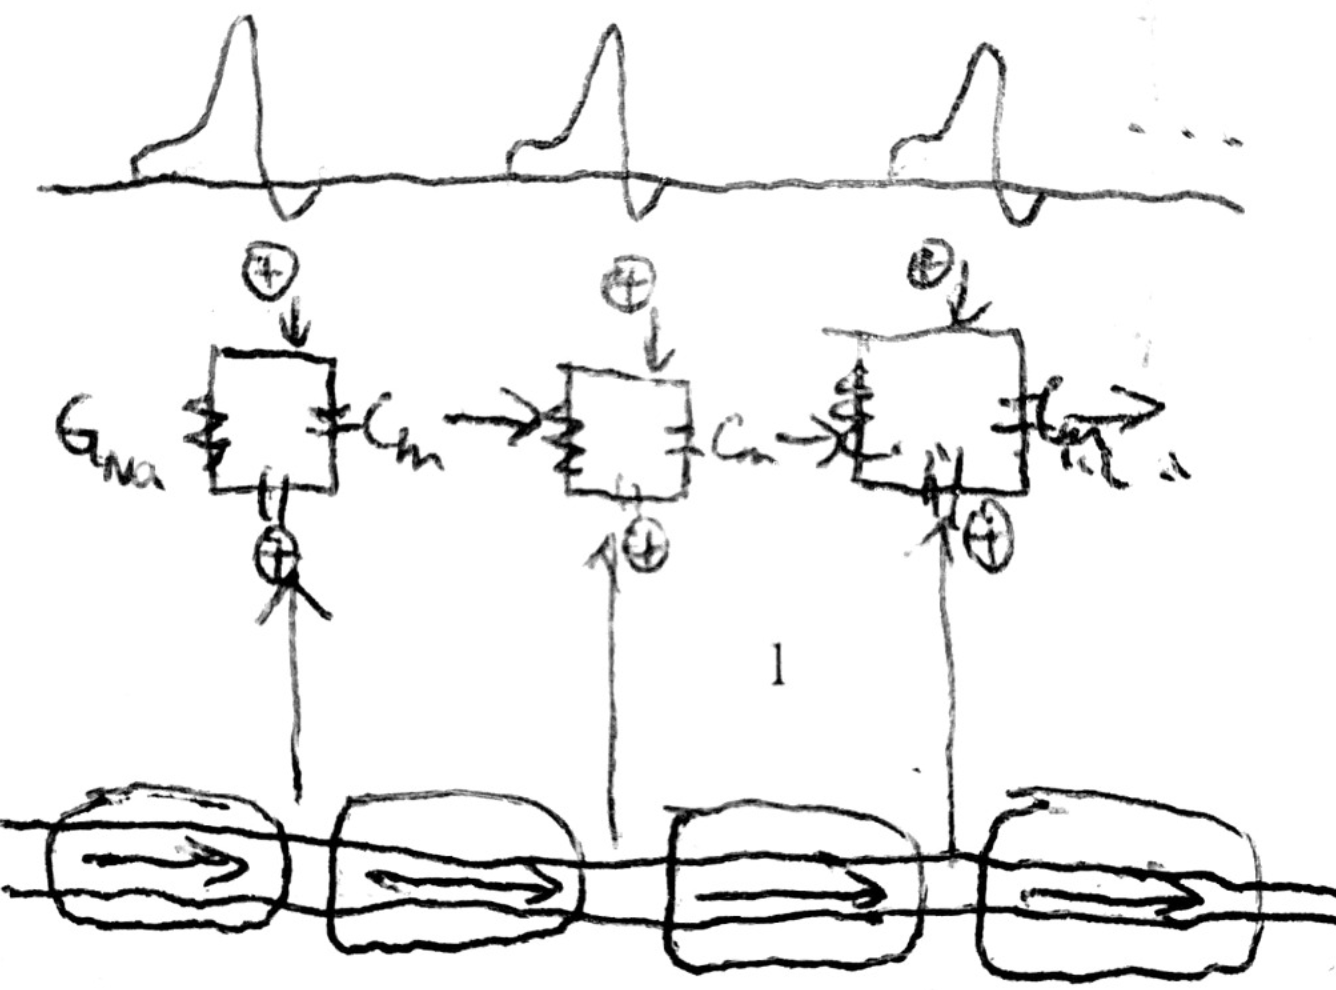
\includegraphics[width=0.5\textwidth]{/Users/jonathansun5/Documents/Fall 2017/MCB 166/Homeworks/Midterm/Screen Shot 2017-10-10 at 10.51.13 AM.png}
\end{center}



\newpage
\item
Sketch the \ch{Na+} and \ch{K+} currents that flow during an action potential. (Hint: Look up how $g_{\ch{Na}}$ and $g_{\ch{K}}$ vary with time during the action potential --- given in the class notes --- and then recall that $I_{\ch{Na}} = g_{\ch{Na}} \left(V - V_{\ch{Na}}\right)$, $I_{\ch{K}} = g_{\ch{K}} \left(V - V_{\ch{K}}\right)$, and that the voltage $V(t)$ is varying according to the action-potential shape. You can do this qualitatively, but justify your answer. A common mistake is to confuse the currents that flow during the action potential with the voltage-clamp currents that flow in response to a depolarizing pulse.
\begin{center}
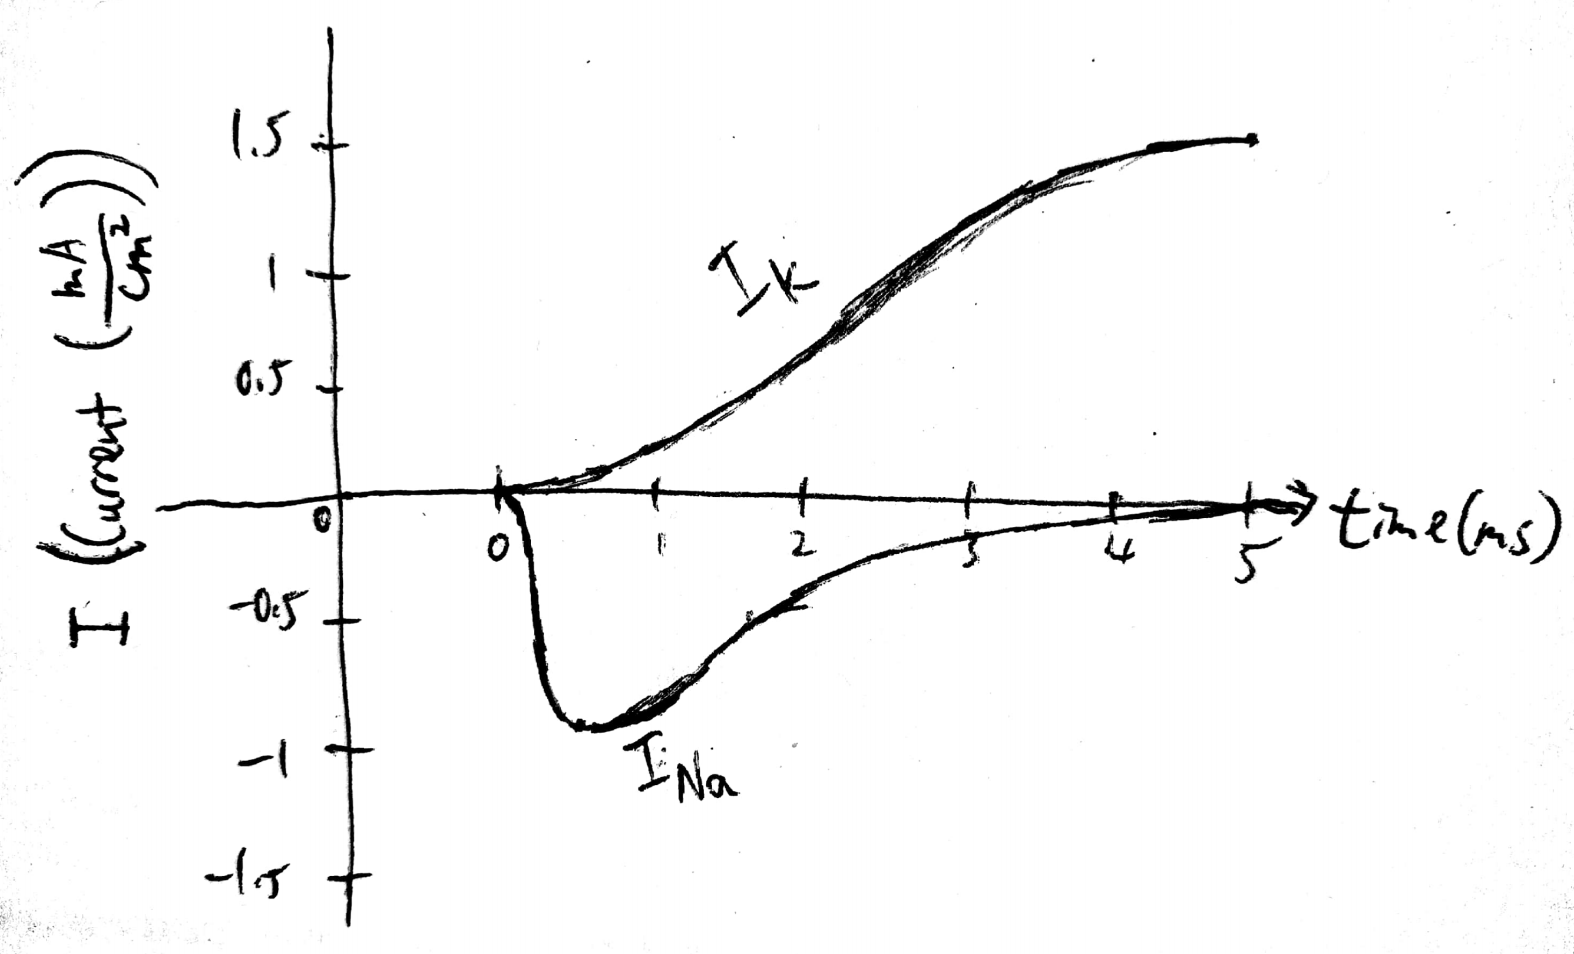
\includegraphics[width=0.75\textwidth]{/Users/jonathansun5/Documents/Fall 2017/MCB 166/Homeworks/Midterm/Screen Shot 2017-10-10 at 5.14.12 AM.png}
\end{center}



\newpage
\item
Explain the following action-potential phenomena in terms of the Hodgkin-Huxley variables, $m$, $h$, and $n$. Write the relevant variable for each of the phenomenon listed below, and explain your choice in a sentence or two.
\begin{enumerate}[label=(\roman*)]
\item
Sharp rise in voltage in response to a short-duration stimulus of $30$ mV above rest.
\vspace*{1\baselineskip}
\\
The relevant variables are $m$ and $h$ since this is describing the rising phase of the action potential. This is when \ch{Na+} channels are opening, which is reflected by the variables $m$ and $h$.



\item
Initial decline in voltage after the action potential reaches its peak.
\vspace*{1\baselineskip}
\\
The relevant variable is $n$ and since this is describing the falling phase of the action potential. This is when \ch{K+} channels are opening, which is reflected by the variable $n$.



\item
Hyperpolarizing voltage for a few msec after the action potential has subsided.
\vspace*{1\baselineskip}
\\
The relevant variable is $n$ since this is describing the hyperpolarization part. This is when \ch{K+} is being expelled, which is reflected by the variable $n$.



\item
Anode-break effect in which a hyperpolarizing conditioning pulse prior to application of the stimulus causes the threshold to get lower.
\vspace*{1\baselineskip}
\\
The relevant variable is $n$ since this is describing the hyperpolarization part. This is when \ch{K+} is being expelled, which is reflected by the variable $n$.
\end{enumerate}
\end{enumerate}



\newpage
\item
\underline{Gated Ion Channels.}
\vspace*{1\baselineskip}
\\
Gated ion channels are membrane proteins capable of undergoing rapid conformation changes between conducting and nonconducting states. Consider a simple channel in which the gating is effected by a single charged group that moves during the conformation change. When the channels are in steady state under an applied transmembrane electric field, the energy difference between the open and closed state is given by
\begin{align*}
\Delta W(V) = -Q_q(V - V_0),
\end{align*}
where $Q_g$ is the effective charge that moves across the membrane during the gating transition, and $\Delta W_{\text{conf}} = Q_g V_0$ represents some intrinsic voltage-independent energy difference between the two conformations.
\begin{enumerate}[label=(\alph*)]
\item
Assume that the open and closed states distributed according to a Boltzmann distribution,
\begin{align*}
N_{\text{open}} / N_{\text{closed}} = \text{exp}(-\Delta W / k T).
\end{align*}
Derive an expression for the steady state voltage dependent conductance for a collection of $N$ gated channels $\left(N = N_{\text{open}} + N_{\text{closed}}\right)$ having a single-channel conductance, $\gamma$ .
\vspace*{1\baselineskip}
\\
To derive the expression I will solve for $G_{\text{ss}}(V)$ from the Boltzmann Ratio:
\begin{align*}
\text{Boltzmann Ratio} = \frac{N_{\text{open}}} {N_{\text{closed}}} = e ^ {- \frac{\Delta W} {k T}}
\end{align*}
Since $N = N_{\text{open}} + N_{\text{closed}}$, we can rearrange it as $N_{\text{closed}} = N - N_{\text{open}}$ and continue:
\begin{align*}
\frac{N_{\text{open}}} {N - N_{\text{open}}} = e ^ {- \frac{\Delta W} {k T}}
\end{align*}
\begin{align*}
N_{\text{open}} = e ^ {- \frac{\Delta W} {k T}} \left(N - N_{\text{open}}\right)
\end{align*}
\begin{align*}
N_{\text{open}} = Ne ^ {- \frac{\Delta W} {k T}} - N_{\text{open}} e ^ {- \frac{\Delta W} {k T}}
\end{align*}
\begin{align*}
N_{\text{open}} + N_{\text{open}} e ^ {- \frac{\Delta W} {k T}} = Ne ^ {- \frac{\Delta W} {k T}}
\end{align*}
\begin{align*}
N_{\text{open}} = \frac{Ne ^ {- \frac{\Delta W} {k T}}} {1 + e ^ {- \frac{\Delta W} {k T}}}
\end{align*}
\begin{align*}
N_{\text{open}} = \frac{N} {e ^ {\frac{\Delta W} {k T}} + 1}
\end{align*}
Since $\Delta W(V) = -Q_q(V - V_0)$:
\begin{align*}
N_{\text{open}} = \frac{N} {e ^ {\frac{-Q_q(V - V_0)} {k T}} + 1}
\end{align*}
\begin{align*}
G_{\text{ss}}(V) = \frac{N_{\gamma}} {1 + e ^ {\frac{-Q_q(V - V_0)} {k T}}}
\end{align*}



\newpage
\item
Sketch the curve of steady-state voltage-dependent conductance, $G_{\text{ss}}(V)$. Indicate the maximum value of $G_{\text{ss}}(V)$, and the voltage $V_0$. What fraction of the channels is open at $V_0$?
\begin{center}
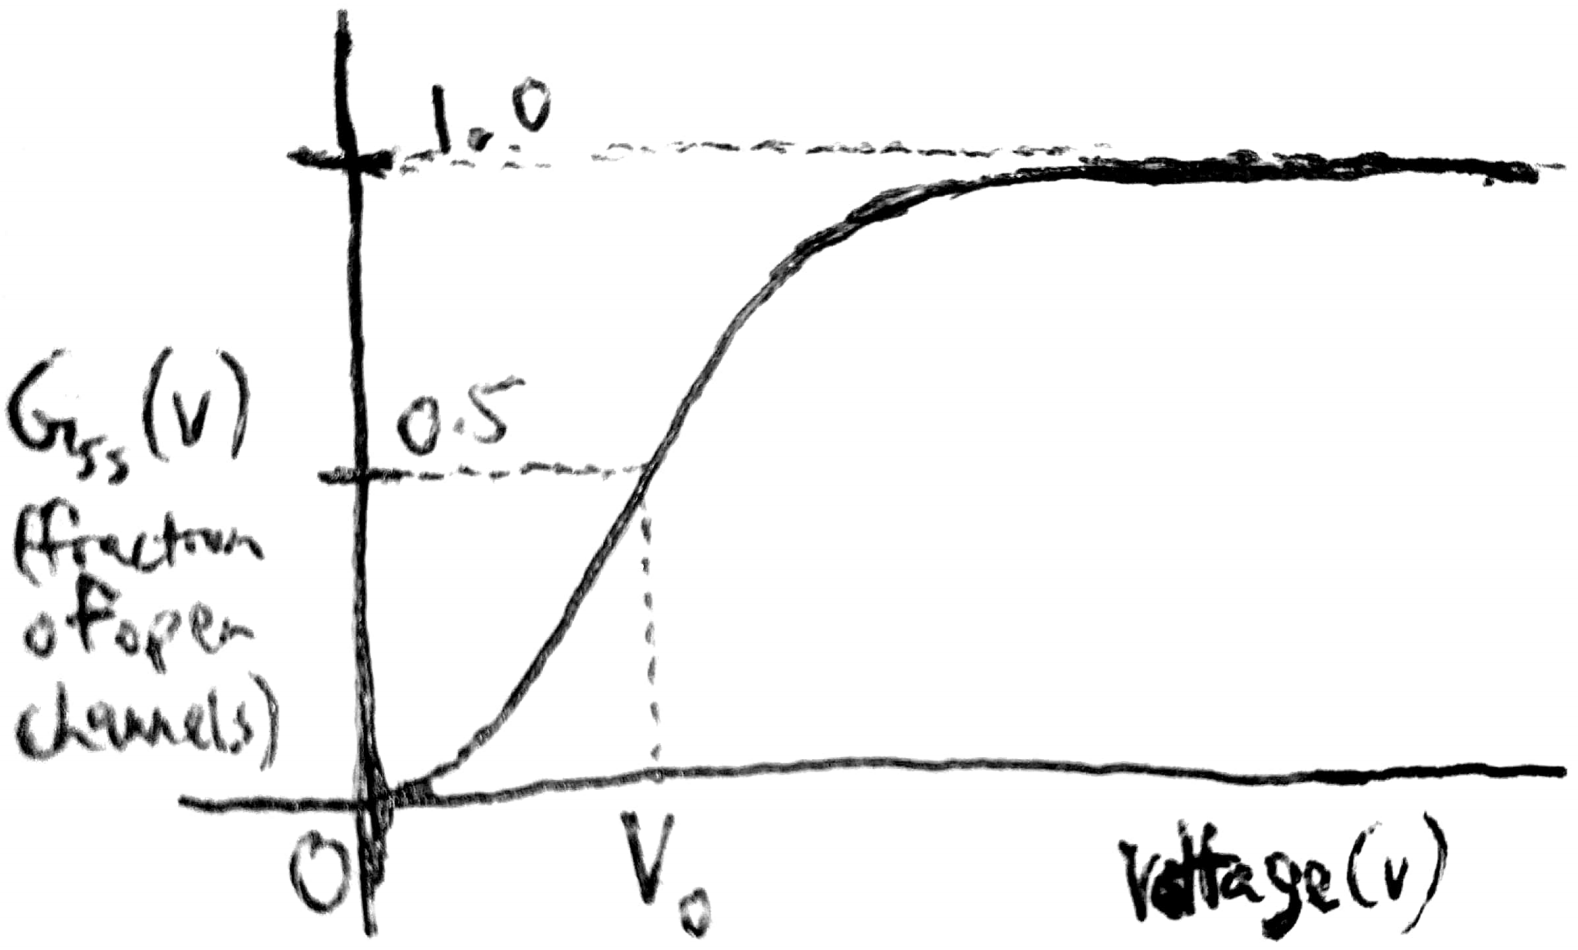
\includegraphics[width=0.75\textwidth]{/Users/jonathansun5/Documents/Fall 2017/MCB 166/Homeworks/Midterm/Screen Shot 2017-10-10 at 8.07.09 AM.png}
\end{center}
The maximum value of $G_{\text{ss}}(V)$ is $1$ and $\frac{1} {2}$ of the channels are open at $V_0$.



\newpage
\item
Say the channel is \ch{Na+} selective, so that the current voltage relation of an open channel is
\begin{align*}
I = \gamma \left(V - V_{\ch{Na}}\right).
\end{align*}
(Note: For this part of the problem, you can assume $\gamma = G_{\text{ss}}(V)$.) \\
Assume $V_0 = 20 \text{mV}$, $k T / Q_g =5 \text{mV}$, $[\ch{Na}]_{\text{I}} = 50 \text{mM}$, $[\ch{Na}]_0 = 500 \text{mM}$. Sketch the steady-state current-voltage curve. Indicate the reversal potential and any region of negative conductance. (ie. $dI / dV < 0$).
\vspace*{1\baselineskip}
\\
Before I can sketch the steady-state current-voltage curve, I first need to calculate $E_{\ch{Na}}$:
\begin{align*}
E_{\ch{Na}} = \frac{R T} {z F} \ln{\left(\frac{[\ch{Na}]_o} {[\ch{Na}]_i}\right)}
\end{align*}
From 2(b), we were given that $\frac{R T} {z F} = 25.9 \text{mV}$ so:
\begin{align*}
E_{\ch{Na}} = 25.9 \text{mV} \ln{\left(\frac{500 \text{mM}} {50 \text{mM}}\right)}
\end{align*}
\begin{align*}
E_{\ch{Na}} = 59.64 \text{mV}
\end{align*}
The reversal potential is $E_{\ch{Na}} = 59.64 \text{mV}$ and the graph below is the sketch of the steady-state current-voltage curve.
\begin{center}
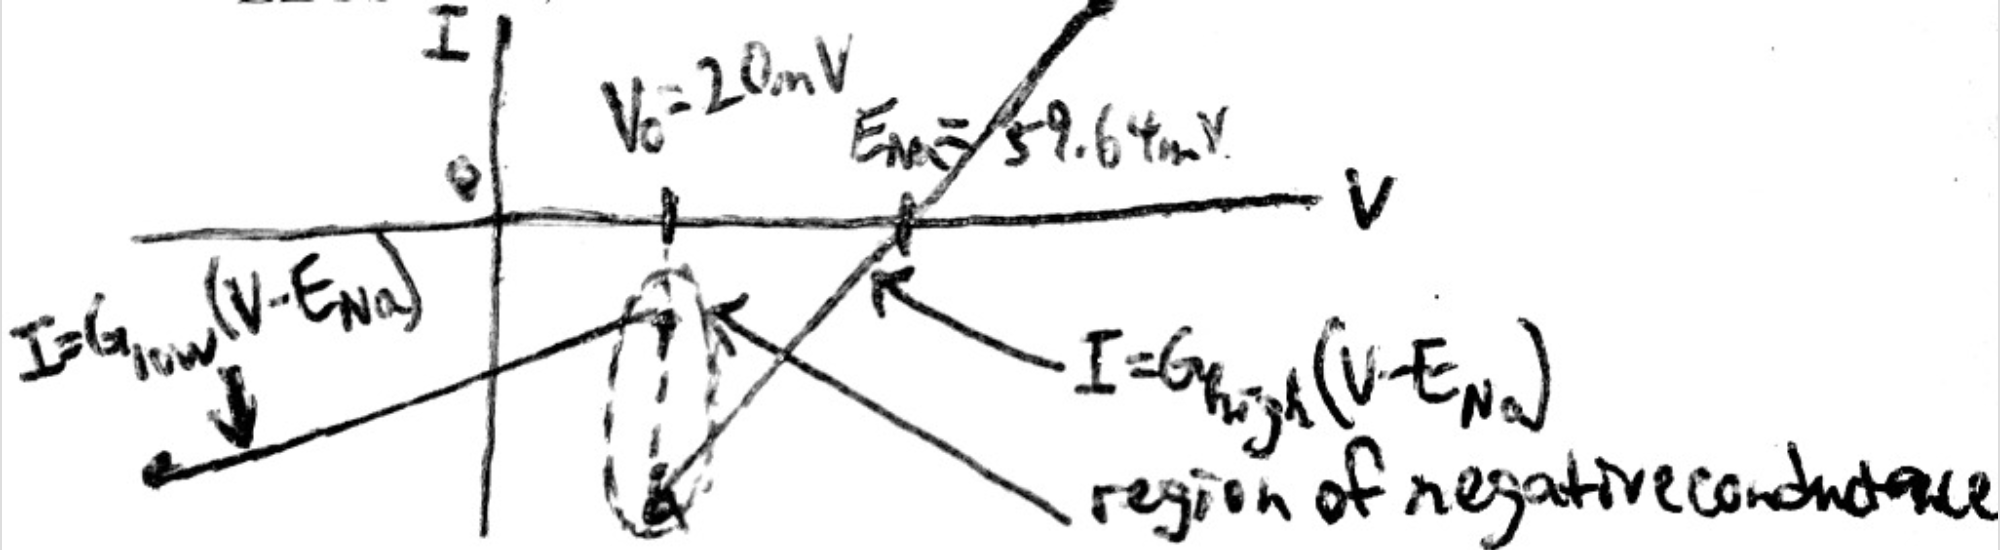
\includegraphics[width=0.75\textwidth]{/Users/jonathansun5/Documents/Fall 2017/MCB 166/Homeworks/Midterm/Screen Shot 2017-10-10 at 9.12.56 AM.png}
\end{center}



\newpage
\item
Briefly state how any region of negative conductance for the current voltage curve of an \ch{Na+} channel is significant for generating an action potential.
\vspace*{1\baselineskip}
\\
Since the $V_{\theta}$ is more negative than $E_{\ch{Na}}$ at the region of negative conductance, this means that \ch{Na+} flows into the cell, which makes the inside of the cell more positively charged and therefore generating an action potential.
\end{enumerate}
\end{enumerate}
\end{document}
